
%===================================================
\chapter{The User Entry Operation}
\label{sec:UserEntry}
%===================================================

\label{sec:userEntry}
This operation is a multi-stage operation and will be presented as 
a number of operations with preconditions on the internal $status$.
The state transition diagram for user authentication and entry is
given in Figure \ref{fig:userEntry}. Before user authentication and
entry the system is in the $quiescent$ state, on completion of the
user authentication and entry the system will return the to
$quiescent$ state.

\begin{figure}[htbp]
  \begin{center}
    \leavevmode
    \resizebox{\textwidth}{!}{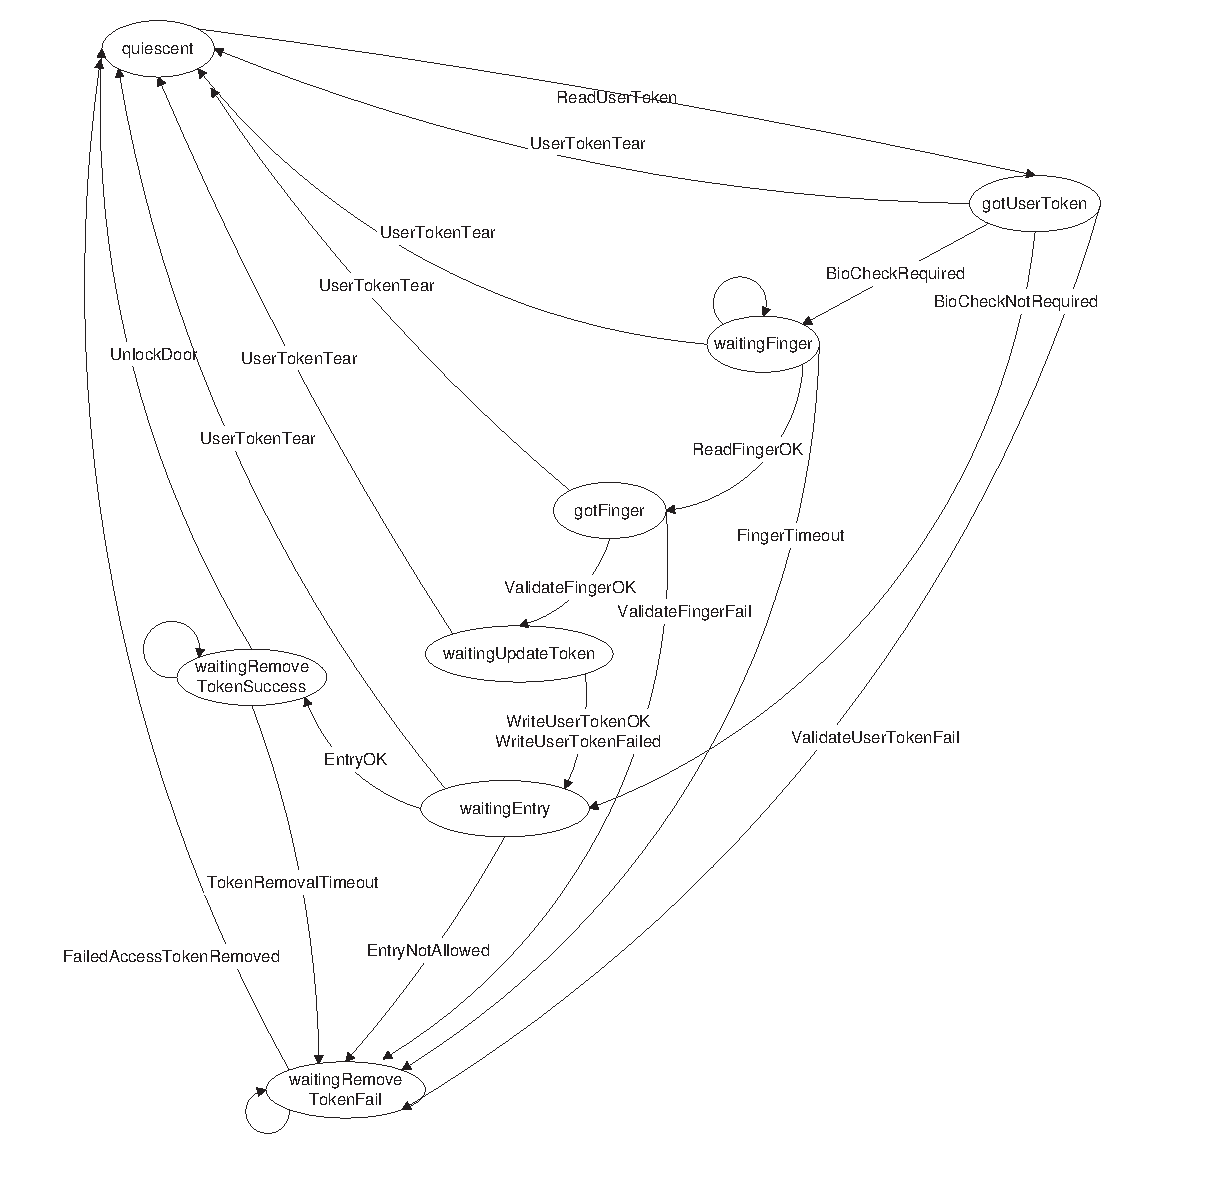
\includegraphics{41_2_entry.eps}}
    \caption{User Authentication and Entry state transitions}
    \label{fig:userEntry}
  \end{center}
\end{figure}

The process of user authentication and entry follows the following
stages:

\begin{itemize}
\item
Before any user attempts access, the system is $quiescent$.
\item
Once the token has been inserted and the information read off,
the status moves to $gotUserToken$, waiting for the system to validate
the token. 
\item
Once the token has been successfully validated the 
status moves to $waitingFinger$,
waiting for the user to give a fingerprint.
\item
Once the fingerprint has been read, the status moves to $gotFinger$,
waiting for the system to validate the fingerprint.
\item
Once a fingerprint has been successfully validated,
the status moves to $waitingUpdateToken$,
waiting to write the Auth Cert to the token.
\item
Once the Auth Cert has been written, the status moves to
$waitingEntry$, where it determines whether the role has
current entry privileges.
\item
If the role has current entry privileges the status moves to
$waitingTokenRemoveSuccess$, where the system waits for 
the token to be removed.
\item
Once the token has been removed
the latch will be unlocked if the role has current access privileges
to the enclave and the ID Station will return to $quiescent$.
\end{itemize}
In the case of a failure in the user validation process the status
moves to  $waitingRemoveTokenFail$, waiting until the token has been removed before returning to a
$quiescent$ state.

This specification separates opening the door from having a valid Auth
Certificate. It is possible for a role to be entitled to enter the
enclave but not use the workstations (for example such clearence might
be given to a buildings maintenance engineer). It is likely that TIS
configurations will ensure that having a valid Auth Certificate will
guarantee that entry to the enclave is permitted. 

\begin{traceunit}{FS.Enclave.ResetScreenMessage}
\end{traceunit}
The message displayed on the screen will indicate that the
system is busy while a user entry is in progress that blocks
administrator activity. Once the user entry activity becomes
non-blocking then an appropriate message is displayed on the screen.

\begin{schema}{ResetScreenMessage}
        \Delta Internal
\\      \Delta Admin
\\      currentScreen, currentScreen' : Screen
\where
        status' \notin \{ quiescent, waitingRemoveTokenFail \} 
\\ \t1 \land currentScreen'.screenMsg = busy
\\      \lor
\\      status' \in \{ quiescent, waitingRemoveTokenFail \}
\\ \t1 \land (enclaveStatus' = enclaveQuiescent \land rolePresent' = \Nil 
\\ \t3          \land currentScreen'.screenMsg = welcomeAdmin
\\ \t2 \lor enclaveStatus' = enclaveQuiescent \land rolePresent' \neq \Nil 
\\ \t3          \land currentScreen'.screenMsg = requestAdminOp
\\ \t2 \lor enclaveStatus' = waitingRemoveAdminTokenFail 
\\ \t3          \land currentScreen'.screenMsg = removeAdminToken
\\ \t2 \lor enclaveStatus' \notin 
        \{ enclaveQuiescent, waitingRemoveAdminTokenFail \} 
\\ \t3          \land currentScreen'.screenMsg = currentScreen.screenMsg)
\end{schema}

The user entry operation leaves much of the $IDStation$ state
unchanged. The context of this operation is summarised:

\begin{schema}{UserEntryContext}
        \Delta IDStation
\\      RealWorldChanges
\also
        \Xi Config
\\      \Xi AdminToken
\\      \Xi KeyStore
\\      \Xi Admin
\\      \Xi Keyboard
\\      \Xi Floppy
\\      \Xi Finger
\also
\\      \Xi TISControlledRealWorld
\also
\\      ResetScreenMessage
\where
        enclaveStatus' = enclaveStatus
\\      status \neq waitingEntry \implies tokenRemovalTimeout' = tokenRemovalTimeout
\end{schema} 

\begin{Zcomment}
\item
The following state components may change $UserToken$,
$DoorLatchAlarm$, $Stats$, $Internal$ and $AuditLog$.
\item
The components of the real world controlled by TIS remain unchanged.
\item
The $tokenRemovalTimeout$ is only updated if the current status is
$waitingEntry$.
\end{Zcomment}

Each of the following sub-operations is performed within the above context.

%----------------------------------------------------------------------
\section{User Token Tears}
%----------------------------------------------------------------------

\begin{traceunit}{FS.UserEntry.UserTokenTorn}
\traceto{ScGainInitial.Suc.Audit}
\traceto{ScGainInitial.Fail.ReadCard}
\traceto{ScProhibitInitial.Suc.Audit}
\traceto{ScProhibitInitial.Fail.ReadCard}
\traceto{ScGainRepeat.Suc.Audit}
\end{traceunit}


During the operation the user may tear his token from the reader
prematurely. There are a number of internal states during which token
removal is deamed erroneous.

If the user tears the Token out before the operation is complete then
the operation is terminated unsuccessfully.

\begin{schema}{UserTokenTorn}
        UserEntryContext
\also
	\Xi UserToken
\\      \Xi DoorLatchAlarm
\\      AddFailedEntryToStats
\also
        AddElementsToLog     
\where
        status \in \{ gotUserToken, waitingUpdateToken,
waitingFinger, gotFinger, waitingEntry \}
\\      userTokenPresence = absent
\also
        currentDisplay' = welcome
\\      status' = quiescent 
\end{schema}

%-------------------------------------------------------------------
\section{Reading the User Token}
%-------------------------------------------------------------------

\begin{traceunit}{FS.UserEntry.TISReadUserToken}
\traceto{ScGainInitial.Ass.Quiescent}
\traceto{ScGainInitial.Suc.Audit}
\traceto{ScGainInitial.Con.NoInterleave}
\traceto{ScProhibitInitial.Ass.Quiescent}
\traceto{ScProhibitInitial.Con.NoInterleave}
\traceto{ScProhibitInitial.Suc.Audit}
\traceto{ScGainRepeat.Ass.Quiescent}
\traceto{ScGainRepeat.Suc.Audit}
\traceto{ScGainRepeat.Con.NoInterleave}
\traceto{FIA\_UID.2.1}
\end{traceunit}

The User Entry operation is initiated when TIS is in a $quiescent$ state
and detects the presence of
a token in the user token reader (which resides outside the enclave). 

A user entry operation may start while the $enclaveStatus$ is
quiescent ($enclaveQuiescent$) or the enclave is waiting for a failed
admin token to be removed.

When the user token is first detected as present, its presence is
audited and the internal status changes. 
No other aspects of the system are modified.

\begin{schema}{ReadUserToken}
        UserEntryContext
\also
        \Xi UserToken
\\	\Xi DoorLatchAlarm
\\      \Xi Stats
\also
        AddElementsToLog
\where
        enclaveStatus \in \{ enclaveQuiescent,
        waitingRemoveAdminTokenFail \}
\also
	status = quiescent
\\	userTokenPresence = present
\also
	currentDisplay' = wait
\\	status' = gotUserToken
\end{schema}

The operation to read the user token is as follows:

\begin{zed}
        TISReadUserToken \defs  ReadUserToken
\end{zed}


%--------------------------------------------------------------------
\section{Validating the User Token}
%--------------------------------------------------------------------
Once TIS has read a user token it must validate the contents of that
token.

A user token is valid for entry into the enclave, without the need for
Biometric checks if the token contains an Authorisation certificate that
cross-checks correctly with the Token ID and the ID certificate, is
current and  both the Authorisation certificate and ID certificate can be
validated using the keys held in the TIS $KeyStore$. 

\begin{schema}{UserTokenWithOKAuthCert}
        KeyStore
\\      UserToken
\\      currentTime : TIME
\where
        currentUserToken \in \ran goodT
\\	\exists TokenWithValidAuth @ 
\\ \t1		(
		goodT(\theta TokenWithValidAuth) = currentUserToken
\\ \t1		\land currentTime \in (\The authCert).validityPeriod
\\ \t1          \land (\exists IDCert @ \theta IDCert = idCert \land CertOK )
\\ \t1          \land (\exists AuthCert @ \theta AuthCert = \The
authCert \land AuthCertOK )  
		)
\end{schema}



A user token is valid for entry into the enclave if the token is
consistent, current and the ID
certificate, Privilege certificate and I\&A certificate can be validated. This is regardless of the
presence or state of the Authorisation certificate. However in this
circumstance biometric checks will be required.

\begin{schema}{UserTokenOK}
        KeyStore
\\      UserToken
\\      currentTime : TIME
\where
 	currentUserToken \in \ran goodT
\\	\exists CurrentToken @ 
\\ \t1		(
		goodT(\theta ValidToken) = currentUserToken
\\ \t1		\land now = currentTime
\\ \t1          \land (\exists IDCert @ \theta IDCert = idCert \land CertOK )
\\ \t1          \land (\exists PrivCert @ \theta PrivCert = privCert
\land CertOK )
\\ \t1          \land (\exists IandACert @ \theta IandACert =
iandACert \land CertOK )  
                )
\end{schema}

\begin{traceunit}{FS.UserEntry.BioCheckNotRequired}
\traceto{ScGainInitial.Ass.GoodAC}
\traceto{ScGainRepeat.Suc.Audit}
\traceto{FCO\_NRO.2.1}
\traceto{FCO\_NRO.2.1}
\traceto{FCO\_NRO.2.3}
\traceto{FDP\_DAU.2.1}
\traceto{FDP\_DAU.2.2}
\end{traceunit}

In the case where there is a
valid Authorisation certificate the biometric checks are bypassed.

\begin{schema}{BioCheckNotRequired}
        UserEntryContext
\also
        \Xi UserToken
\\      \Xi DoorLatchAlarm        
\\      \Xi Stats
\also
        AddElementsToLog
\where
        status = gotUserToken
\\      userTokenPresence = present
\also
        UserTokenWithOKAuthCert
\also
        status' = waitingEntry
\\      currentDisplay' = wait
\end{schema}
\begin{Zcomment}
\item
The $userTokenValidElement$ is the audit entry recording that the
token has been succesfully validated.
\item 
The $authCertValidElement$ is the audit entry recording that the
token has a valid authorisation certificate.
\end{Zcomment}


\begin{traceunit}{FS.UserEntry.BioCheckRequired}
\traceto{ScGainInitial.Ass.ValidUser}
\traceto{ScGainInitial.Ass.PoorAC}
\traceto{ScGainInitial.Suc.Audit}
\traceto{FCO\_NRO.2.1}
\traceto{FCO\_NRO.2.1}
\traceto{FCO\_NRO.2.3}
\traceto{FDP\_DAU.2.1}
\traceto{FDP\_DAU.2.2}
\end{traceunit}


The biometric checks are only required if the Authorisation
Certificate is not present or not valid. In this case the remaining
certificates on the card must be checked.



\begin{schema}{BioCheckRequired}
        UserEntryContext
\also
        \Xi UserToken
\\      \Xi DoorLatchAlarm        
\\      \Xi Stats
\also
        AddElementsToLog
\where
        status = gotUserToken
\\      userTokenPresence = present
\also
        \lnot UserTokenWithOKAuthCert \land UserTokenOK
\also
	currentDisplay' = insertFinger
\\	status' = waitingFinger
\end{schema}


\begin{zed}
ValidateUserTokenOK \defs BioCheckRequired \lor BioCheckNotRequired
\end{zed}

\begin{traceunit}{FS.UserEntry.ValidateUserTokenFail}
\traceto{ScGainInitial.Fail.ReadCard}
\traceto{ScProhibitInitial.Ass.FalseUser}
\traceto{ScProhibitInitial.Ass.PoorAC}
\traceto{ScProhibitInitial.Suc.Audit}
\traceto{ScProhibitInitial.Fail.ReadCard}
\traceto{ScGainRepeat.Fail.ReadCard}
\end{traceunit}



There are lots of things that may go wrong with validation of the user
token. In each case the system will terminate the operation unsuccessfully.

\begin{schema}{ValidateUserTokenFail}
        UserEntryContext
\also
        \Xi UserToken
\\      \Xi DoorLatchAlarm
\\      \Xi Stats       
\also
        AddElementsToLog
\where
        status = gotUserToken
\\      userTokenPresence = present
\also
        \lnot UserTokenWithOKAuthCert \land \lnot UserTokenOK 
\also
        currentDisplay' = removeToken
\\      status' = waitingRemoveTokenFail
\end{schema}

\begin{zed}
        TISValidateUserToken \defs ValidateUserTokenOK \lor
        ValidateUserTokenFail 
\\ \t4 \lor
        [~UserTokenTorn | status = gotUserToken ]
\end{zed}

%-----------------------------------------------------------------
\section{Reading a fingerprint}
%----------------------------------------------------------------

\begin{traceunit}{FS.UserEntry.ReadFingerOK}
\traceto{ScGainInitial.Suc.Audit}
\traceto{ScProhibitInitial.Suc.Audit}
\end{traceunit}

A finger will be read if the system is currently waiting for it and
the user Token is in place.

\begin{schema}{ReadFingerOK}
        UserEntryContext
\also
        \Xi DoorLatchAlarm
\\	\Xi UserToken
\\      \Xi Stats
\also
        AddElementsToLog
\where
	status = waitingFinger
\\	fingerPresence = present
\\      userTokenPresence = present
\also
\\	currentDisplay' = wait
\\	status' = gotFinger
\end{schema}

\begin{traceunit}{FS.UserEntry.NoFinger}
\end{traceunit}


If there is no finger present then either nothing happens, since we
have not allowed sufficient attempts to get and validate a finger...

\begin{schema}{NoFinger}
        \Xi IDStation
\\      RealWorldChanges
\also
        \Xi TISControlledRealWorld
\where
        status = waitingFinger
\\      fingerPresence = absent
\\      userTokenPresence = present
\end{schema}


\begin{traceunit}{FS.UserEntry.FingerTimeout}
\traceto{ScGainInitial.Fail.Fingerprint}
\traceto{ScProhibitInitial.Suc.Audit}
\traceto{ScProhibitInitial.Fail.Fingerprint}
\end{traceunit}

...or TIS may have tried to obtain a valid finger for too
long, in which case the user is requested to remove the token and 
the operation is terminated unsuccessfully. Abstractly this  decision
is made non-deterministically.

\begin{schema}{FingerTimeout}
        UserEntryContext
\also
        \Xi UserToken
\\      \Xi DoorLatchAlarm
\\      \Xi Stats       
\also
        AddElementsToLog
\where
        status = waitingFinger
\\      userTokenPresence = present
\also
        currentDisplay' = removeToken
\\      status' = waitingRemoveTokenFail
\end{schema}

\begin{zed}
        TISReadFinger \defs ReadFingerOK \lor
        FingerTimeout \lor NoFinger 
\\ \t4  \lor [~ UserTokenTorn | status = waitingFinger ~]
\end{zed}

%-------------------------------------------------------------
\section{Validating a fingerprint}
%-------------------------------------------------------------

\begin{traceunit}{FS.UserEntry.ValidateFingerOK}
\traceto{ScGainInitial.Ass.ValidUser}
\traceto{ScGainInitial.Suc.Audit}
\end{traceunit}


A finger must match the template information extracted from the
userToken for it to be considered acceptable. The match criterion is
not modelled formally here athough it is necessary for the 
fingerprint to at least be good.

\begin{schema}{FingerOK}
        Finger
\\      UserToken
\where
        currentFinger \in \ran goodFP
\end{schema}

Within this specification the fingerprint will non-deterministically
match or not, assuming it is good.

The fingerprint being successfully validated is a prerequisite for
generating an authorisation certificate and adding it to the user token.
Validating the fingerprint is performed first.

\begin{schema}{ValidateFingerOK}
	UserEntryContext
\also
	\Xi DoorLatchAlarm
\\      \Xi UserToken
\also
        AddSuccessfulBioCheckToStats
\\      AddElementsToLog
\where
	status = gotFinger
\\      userTokenPresence = present
\also
        FingerOK
\also
	status' = waitingUpdateToken
\\	currentDisplay' = wait
\end{schema}


\begin{traceunit}{FS.UserEntry.ValidateFingerFail}
\traceto{ScGainInitial.Fail.Fingerprint}
\traceto{ScProhibitInitial.Ass.FalseUser}
\traceto{ScProhibitInitial.Suc.Audit}
\end{traceunit}


If the fingerprint is not successfully validated the user is asked to
remove their token and the entry attempt is terminated. 
The biometric check failure is recorded.

\begin{schema}{ValidateFingerFail}
        UserEntryContext
\also
	\Xi UserToken
\\      \Xi DoorLatchAlarm
\also      
        AddFailedBioCheckToStats
\\      AddElementsToLog
\where
        status = gotFinger
\\      userTokenPresence = present
\also
        currentDisplay' = removeToken
\\      status' = waitingRemoveTokenFail
\end{schema}

\begin{zed}
        TISValidateFinger \defs ValidateFingerOK \lor ValidateFingerFail
\\ \t4  \lor [~ UserTokenTorn | status = gotFinger ~]
\end{zed}

%---------------------------------------------------------------------
\section{Writing the User Token}
%----------------------------------------------------------------------


\begin{traceunit}{FS.UserEntry.WriteUserTokenOK}
\traceto{ScGainInitial.Suc.GoodAC}
\traceto{ScGainInitial.Suc.PersistCerts}
\traceto{ScGainInitial.Suc.Audit}
\end{traceunit}

An attempt is made to write this certificate to the token. The write of
the authorisation certificate may be successful...

\begin{schema}{WriteUserTokenOK}
	UserEntryContext
\also
	\Xi DoorLatchAlarm
\\      \Xi Stats
\also
        AddElementsToLog
\\      AddAuthCertToUserToken
\where
	status = waitingUpdateToken
\\      userTokenPresence = present
\also
        status' = waitingEntry
\\      currentDisplay' = wait
\end{schema}


\begin{traceunit}{FS.UserEntry.WriteUserTokenFail}
\traceto{ScGainInitial.Fail.WriteCard}
\end{traceunit}

... or may fail. The failure case models circumstances where the TIS
can detect the failure, through a write failure for instance. 
As there is no read back of the authorisation certificate we cannot
guarantee that the audit log indicating a successful write means that
the token contains the authorisation certificate. The user will still
subsequently be admitted to the enclave if the conditions are correct. 

\begin{schema}{WriteUserTokenFail}
	UserEntryContext
\also
	\Xi DoorLatchAlarm
\\      \Xi Stats
\also
        AddElementsToLog
\\      AddAuthCertToUserToken
\where
	status = waitingUpdateToken
\\      userTokenPresence = present
\also
        status' = waitingEntry
\\      currentDisplay' = tokenUpdateFailed
\end{schema}


Abstractly, whether the authorisation certificate is successfully
written or not is non-deterministic.   

The failure will actually happen during the physical write to the
token, during $UpdateUserToken$. However, as the
operations $WriteUserToken$ and $UpdateUserToken$ are both used to
build the atomic operation $TISWriteUserToken$, the non-deterministic 
failure still happens sometime within this atomic operation.

\begin{zed}
WriteUserToken \defs WriteUserTokenOK \lor WriteUserTokenFail
\end{zed}

\begin{zed}
        TISWriteUserToken \defs (
        WriteUserToken \semi UpdateUserToken )
\\ \t4          \lor [~ UserTokenTorn | status = waitingUpdateToken ~] 
\end{zed}



%------------------------------------------------------------
\section{Validating Entry}
%------------------------------------------------------------

The door will only be unlocked if the current TIS configuration allows
the user to enter the enclave at this time. It is likely that TIS
configurations will ensure that having a valid Auth Certificate will
guarantee that entry to the enclave is permitted, but such a
constraint is not specified here. 

TIS checks to ensure that the current configuration allows the user to
enter the enclave:


\begin{schema}{UserAllowedEntry}
        UserToken
\\      Config
\\      currentTime: TIME
\where
        (\exists ValidToken @ 
\\ \t1  goodT (\theta ValidToken) = currentUserToken
\\ \t1  \land currentTime \in entryPeriod~ privCert.role~
privCert.clearance.class )
\\ \lor
        (\exists TokenWithValidAuth @ 
\\ \t1 goodT(\theta TokenWithValidAuth) = currentUserToken 
\\ \t1 \land currentTime \in entryPeriod~
        (\The authCert).role~ (\The authCert).clearance.class)
\end{schema}


\begin{traceunit}{FS.UserEntry.EntryOK}
\end{traceunit}


Only if entry is permitted at the current time will the user be
admitted to the enclave.

\begin{schema}{EntryOK}
        UserEntryContext
\also
        \Xi DoorLatchAlarm
\\      \Xi UserToken
\\      \Xi Stats
\also
        AddElementsToLog
\where
        status = waitingEntry
\\      userTokenPresence = present
\also
        UserAllowedEntry
\also
        currentDisplay' = openDoor
\\      status' = waitingRemoveTokenSuccess
\\      tokenRemovalTimeout' = currentTime + tokenRemovalDuration
\end{schema}

\begin{traceunit}{FS.UserEntry.EntryNotAllowed}
\end{traceunit}

If the user is not allowed entry at this time they will be
requested to remove their token.

\begin{schema}{EntryNotAllowed}
        UserEntryContext
\also
        \Xi DoorLatchAlarm
\\      \Xi UserToken
\\      \Xi Stats       
\also
        AddElementsToLog
\where
        status = waitingEntry
\\      userTokenPresence = present
\also
        \lnot UserAllowedEntry
\also
        currentDisplay' = removeToken
\\      status' = waitingRemoveTokenFail
\\      tokenRemovalTimeout' = tokenRemovalTimeout
\end{schema}

\begin{zed}
        TISValidateEntry \defs EntryOK
\\ \t4          \lor EntryNotAllowed
\\ \t4          \lor [~ UserTokenTorn | status = waitingEntry ~] 
\end{zed}


%------------------------------------------------------------
\section{Unlocking the Door}
%------------------------------------------------------------

\begin{traceunit}{FS.UserEntry.UnlockDoorOK}
\traceto{ScGainInitial.Suc.UserCard}
\traceto{ScGainInitial.Suc.UserIn}
\traceto{ScGainInitial.Suc.Audit}
\traceto{ScGainRepeat.Suc.UserCard}
\traceto{ScGainRepeat.Suc.UserIn}
\traceto{ScGainRepeat.Suc.Audit}
\end{traceunit}


The door will only be unlocked once the user has removed their token.
This helps remind the user to take their token with them.

\begin{schema}{UnlockDoorOK}
        UserEntryContext
\also
      \Xi UserToken
\also
        UnlockDoor
\\      AddSuccessfulEntryToStats
\\      AddElementsToLog
\where
        status = waitingRemoveTokenSuccess
\\      userTokenPresence = absent
\also
        currentDisplay' = doorUnlocked
\\      status' = quiescent
\end{schema}

\begin{traceunit}{FS.UserEntry.WaitingTokenRemoval}
\end{traceunit}

The system will wait indefinitely for a token to be removed, however
the system will deny entry to a user who takes too long to extract
their token.

\begin{schema}{WaitingTokenRemoval}
        \Xi IDStation
\\      RealWorldChanges
\also
        \Xi TISControlledRealWorld
\where
        status \in \{ waitingRemoveTokenSuccess, 
waitingRemoveTokenFail \}
\\      status = waitingRemoveTokenSuccess \implies currentTime \leq tokenRemovalTimeout 
\\      userTokenPresence = present
\end{schema}

\begin{traceunit}{FS.UserEntry.TokenRemovalTimeout}
\end{traceunit}

If the user waits too long to remove their token then this is logged
and the system continues to wait for the token to be removed but will
no longer allow access to the enclave.

\begin{schema}{TokenRemovalTimeout}
        UserEntryContext
\also
        \Xi DoorLatchAlarm
\\      \Xi UserToken
\\      \Xi Stats       
\also
        AddElementsToLog
\where
        status = waitingRemoveTokenSuccess
\\      currentTime > tokenRemovalTimeout 
\\      userTokenPresence = present
\also
        status' = waitingRemoveTokenFail
\\      currentDisplay' = removeToken
\end{schema}


\begin{zed}
        TISUnlockDoor \defs UnlockDoorOK 
\\      \t2 \lor [ WaitingTokenRemoval |status =
waitingRemoveTokenSuccess ]
\\      \t2 \lor TokenRemovalTimeout
\end{zed}
 
%------------------------------------------
\section{Terminating a failed access}
%------------------------------------------

\begin{traceunit}{FS.UserEntry.FailedAccessTokenRemoved}
\traceto{ScGainInitial.Suc.Audit}
\traceto{ScProhibitInitial.Suc.UserCard}
\traceto{ScProhibitInitial.Suc.Audit}
\end{traceunit}

If an access attempt has failed the system waits for the token to be
removed before a new user entry operation can commence. Once the token has been
removed a new user entry may start.

The operations in the enclave are not blocked on the presence of a
failed user token in the token reader. 

\begin{schema}{FailedAccessTokenRemoved}
        UserEntryContext
\also
	\Xi UserToken
\\      \Xi DoorLatchAlarm
\also
        AddFailedEntryToStats
\\      AddElementsToLog
\where
        status = waitingRemoveTokenFail
\\      userTokenPresence = absent
\also
        currentDisplay' = welcome
\\      status' = quiescent
\end{schema}

\begin{zed}
        TISCompleteFailedAccess \defs FailedAccessTokenRemoved 
\\      \t2     \lor [ WaitingTokenRemoval | status = waitingRemoveTokenFail ] 
\end{zed}

%..........................................
\section{The Complete User Entry}
%..........................................

\begin{traceunit}{FS.UserEntry.TISUserEntryOp}
\traceto{FIA\_UAU.7.1}
\end{traceunit}

The complete authentication process, triggered by TIS reading a User
Token, involves validating the user Token, reading and validating the
fingerprint, 
writing an authorisation certificate to the user token, waiting for
the user to remove the token, opening the door to the enclave and
in the case of a failure waiting for the system to
be in a state where it can admit another user.

\begin{zed}
        TISUserEntryOp \defs TISReadUserToken \lor TISValidateUserToken \lor TISReadFinger \lor
                TISValidateFinger 
\\ \t4          \lor TISWriteUserToken \lor  TISValidateEntry \lor TISUnlockDoor \lor
                TISCompleteFailedAccess 
\end{zed}


